\documentclass[12pt,a4paper,twoside]{book}
\usepackage{graphicx}
\usepackage{setspace} % espaciado doble para texto, simple para pies de página, subtítulos, etc.
\usepackage{natbib} % sustituto de 'hypernat' que funciona en Windows.
\usepackage[spanish]{babel}
\usepackage[utf8]{inputenc}
\usepackage{color}
\usepackage{hhline} % estilos extendidos para tablas
\usepackage{multirow}
\usepackage{subfigure}
\usepackage{acronym}
\usepackage{hyperref}
\usepackage{amsmath,amssymb}
\usepackage{fancyhdr}
\usepackage{epsfig, amsmath}
\usepackage{algorithm}
\usepackage{algorithmic}
\usepackage[T1]{fontenc}
\usepackage{lmodern}
\usepackage{microtype}

% configuraciones generales
\hypersetup{
linktocpage=true,
colorlinks=true,
linkcolor=blue,
citecolor=blue,
}
\definecolor{Hgray}{gray}{0.6}

\newenvironment{definition}[1][Definición]{\begin{trivlist}
\item[\hskip \labelsep {\bfseries #1}]}{\end{trivlist}}

\setlength{\topmargin}{0cm}
\setlength{\textheight}{23cm}
\setlength{\textwidth}{17cm}
\setlength{\oddsidemargin}{0cm}
\setlength{\evensidemargin}{0cm}
\setlength{\headheight}{1cm}

% indica que las 'sub-sub-secciones' están numeradas y aparecen en el índice
\setcounter{secnumdepth}{3}
\setcounter{tocdepth}{2}

% configuraciones para código
\renewcommand{\algorithmicrequire}{\textbf{Entrada:}}
\renewcommand{\algorithmicensure}{\textbf{Salida:}}

%%%%%%%%%%%%
% DOCUMENTO %
%%%%%%%%%%%%
\begin{document}

\setcounter{section}{0} % Restablece el contador de sección a 0 al inicio del documento
\renewcommand{\thesection}{\arabic{section}} % Cambia el esquema de numeración de sección

\pagenumbering{arabic}

\hypersetup{pageanchor=true}

% portada
\newpage
\thispagestyle{empty}

\baselineskip 2em

%\vspace*{1cm}

\centerline{
\includegraphics[width=0.6\textwidth]{images/UOC-logo}}
\begin{center}
\textsc{Universitat Oberta de Catalunya (UOC) \\
 Máster Universitario en Ciencia de Datos (\textit{Data Science})\\}

%\centerline {\pic{UOC}{4cm}}

\vspace*{1.5cm}

\textsc{\Large TRABAJO FINAL DE MÁSTER}

\vspace*{0.5cm}

\textsc{\large Área: Reinforced Learning}


%\textbf{\Huge VirtualTechLab Model: }

\vspace*{2.0cm}

\textbf{\Large Impacto de la complejidad de las observaciones en el rendimiento de algoritmos de Aprendizaje por Refuerzo en un entorno Pacman}

\vspace{2.5cm}
\baselineskip 1em

\baselineskip 2em
-----------------------------------------------------------------------------\\
Autor:      Alejandro Suau Ruiz\\
Tutor:      Marc Borras Camarasa\\
Profesor:   David Masip Rodó\\
-----------------------------------------------------------------------------\\
\vspace*{1.5cm}
Palma de Mallorca, \today

\end{center}

\newpage
\pagestyle{empty}
\hfill

\newpage
% resumen
\hypersetup{pageanchor=false}
\pagenumbering{roman} 
\setcounter{page}{1} 
\pagestyle{plain}

%%%%%%%%%%%%%%%%
%%% CREDITOS %%%
%%%%%%%%%%%%%%%%
\chapter*{Créditos/Copyright}

Una página con la especificación de créditos/copyright para el proyecto (ya sea aplicación por un lado y documentación por el otro, o unificadamente), así como la del uso de marcas, productos o servicios de terceros (incluidos códigos fuente). Si una persona diferente al autor colaboró en el proyecto, tiene que quedar explicitada su identidad y qué hizo.

A continuación se ejemplifica el caso más habitual, aunque se puede modificar por cualquier otra alternativa:

\vspace{1cm}

\begin{figure}[ht]
    \centering
	
\includegraphics[scale=1]{images/license.png}
\end{figure}

Esta obra está sujeta a una licencia de Reconocimiento -  NoComercial - SinObraDerivada

\href{https://creativecommons.org/licenses/by-nc-nd/3.0/es/}{3.0 España de CreativeCommons}.

%%%%%%%%%%%%%
%%% FICHA %%%
%%%%%%%%%%%%%
\chapter*{FICHA DEL TRABAJO FINAL}

\begin{table}[ht]
	\centering{}
	\renewcommand{\arraystretch}{2}
	\begin{tabular}{r | l}
		\hline
		Título del trabajo: & Impacto de la complejidad de las observaciones en el rendimiento de algoritmos de Aprendizaje por Refuerzo en un entorno Pacman\\
		\hline
        Nombre del autor: & Alejandro Suau Ruiz\\
		\hline
        Nombre del colaborador/a docente: & Marc Borras Camarasa\\
		\hline
        Nombre del PRA: & David Masip Rodó\\
		\hline
        Fecha de entrega (mm/aaaa): & 01/2026\\
		\hline
        Titulación o programa: & Máster Universitario de Data Science\\
		\hline
        Área del Trabajo Final: & Reinforced Learning\\
		\hline
        Idioma del trabajo: & Español\\
		\hline
        Palabras clave & Aprendizaje por refuerzo, Complejidad del estado, Pacman\\
		\hline
	\end{tabular}
\end{table}

%%%%%%%%%%%%%%%%%%%
%%% DEDICATORIA %%%
%%%%%%%%%%%%%%%%%%%
\chapter*{Dedicatoria/Cita}

Breves palabras de dedicatoria y/o una cita.

%%%%%%%%%%%%%%%%%%%
%%% Agradecimientos %%%
%%%%%%%%%%%%%%%%%%%
\chapter*{Agradecimientos}

Si se considera oportuno, mencionar a las personas, empresas o instituciones que hayan contribuido en la realización de este proyecto.

%%%%%%%%%%%%%%%%
%%% ABSTRACT%%%
%%%%%%%%%%%%%%%%
\chapter*{Abstract}
\addcontentsline{toc}{chapter}{Abstract}

\onehalfspacing

This work investigates how the complexity of state representation affects the performance of reinforcement learning algorithms in a simplified Pacman environment. The central idea is that an agent’s success depends not only on the algorithm itself but also on the quality and richness of the information it receives from the environment. To analyze this, we designed a set of progressively more complex observation spaces, ranging from the basic positions of the player and the ghost to configurations that include the presence and duration of power-ups and the distribution of coins across quadrants.
Experiments were carried out using widely adopted algorithms such as PPO, A2C, and DQN, implemented with the Stable-Baselines3 library. Controlled training with different random seeds and consistent performance metrics allowed us to compare both learning speed and the stability of the learned policies.
The results show that increasing state complexity does not always lead to better performance: in some cases, the additional information introduces noise and hinders convergence. However, for specific configurations, the agent was able to exploit the extra information to achieve more robust behavior.
In conclusion, the project highlights the importance of observation design in the success of reinforcement learning agents, stressing the need to balance simplicity and expressiveness depending on the task and the chosen algorithm.

\vspace{1.5cm}

\textbf{Keywords}: Reinforcement learning, State complexity, Pacman, Stable-Baselines3, Gymnasium

%%%%%%%%%%%%%%%%
%%% RESUMEN    %%%
%%%%%%%%%%%%%%%%

\chapter*{Resumen}
\addcontentsline{toc}{chapter}{Resumen}

\onehalfspacing

Este trabajo explora cómo la complejidad de la representación del estado influye en el rendimiento de los algoritmos de aprendizaje por refuerzo en un entorno simplificado de Pacman. Partimos de la premisa de que un agente no aprende únicamente por el algoritmo empleado, sino también por la calidad y la riqueza de la información que percibe del entorno. Para analizarlo, hemos diseñado un conjunto de observaciones progresivamente más complejas, desde la posición básica de jugador y fantasma, hasta configuraciones que incluyen la presencia y duración de comodines o la distribución de monedas por cuadrantes.
La experimentación se ha llevado a cabo con algoritmos ampliamente utilizados, como PPO, A2C y DQN, implementados con la librería Stable-Baselines3. Se han realizado entrenamientos controlados con semillas distintas y métricas de rendimiento homogéneas, lo que ha permitido comparar tanto la velocidad de aprendizaje como la estabilidad de las políticas aprendidas.
Los resultados muestran que un aumento en la complejidad del estado no garantiza siempre un mejor desempeño: en ciertos casos, la mayor riqueza de información introduce ruido y dificulta la convergencia. Sin embargo, para determinadas configuraciones el agente logra aprovechar la información adicional y alcanzar un comportamiento más robusto.
En conclusión, el proyecto confirma la relevancia del diseño de observaciones en el éxito de un agente de aprendizaje por refuerzo, subrayando la necesidad de equilibrar simplicidad y expresividad en función del objetivo y del algoritmo empleado.


\vspace{1.5cm}

\textbf{Palabras clave}: Aprendizaje por refuerzo, Complejidad del estado, Pacman, Stable-Baselines3, Gymnasium
\newpage

\pagestyle{fancy}
\renewcommand{\chaptermark}[1]{ \markboth{#1}{}}
\renewcommand{\sectionmark}[1]{\markright{ \thesection.\ #1}}
\lhead[\fancyplain{}{\bfseries\thepage}]{\fancyplain{}{\bfseries\rightmark}}
\rhead[\fancyplain{}{\bfseries\leftmark}]{\fancyplain{}{\bfseries\thepage}}
\cfoot{}

% tabla de contenidos
\cleardoublepage
\phantomsection
\addcontentsline{toc}{chapter}{Índice}
\tableofcontents
% lista de figuras
\cleardoublepage
\phantomsection
\addcontentsline{toc}{chapter}{Lista de Figuras}
\listoffigures
% lista de tablas
\cleardoublepage
\phantomsection
\addcontentsline{toc}{chapter}{Lista de Tablas}
\listoftables

\thispagestyle{empty}

\pagenumbering{arabic}

\pagestyle{fancy}
\renewcommand{\chaptermark}[1]{ \markboth{#1}{}}
\renewcommand{\sectionmark}[1]{\markright{ \thesection.\ #1}}
\lhead[\fancyplain{}{\bfseries\thepage}]{\fancyplain{}{\bfseries\rightmark}}
\rhead[\fancyplain{}{\bfseries\leftmark}]{\fancyplain{}{\bfseries\thepage}}
\cfoot{}

\onehalfspacing

% capítulos del documento
\section{Introducción}

Esta plantilla pretende ser una guía para los estudiantes. Esta plantilla se puede adaptar a las necesidades específicas de cada proyecto si el supervisor del proyecto está de acuerdo con los cambios.

\begin{figure}[h]
\centering
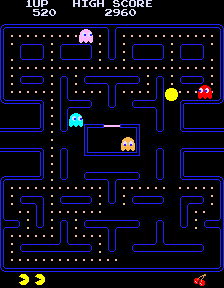
\includegraphics[width=0.5\textwidth]{./figs/image1.png}
\caption{Ejemplo de figura. Será indexada en la “Lista de Figuras”.}
\label{fig:figura_ejemplo}
\end{figure}

\subsection{Contexto y motivación}

Punto de partida del proyecto (¿Cuál es el problema que necesita ser resuelto? ¿Por qué es un tema relevante? ¿Cómo se está resolviendo el problema actualmente?) y descripción de la contribución (¿Qué resultado se espera obtener?)

\subsection{Objetivos}

Listado de los objetivos a alcanzar en este proyecto.

\subsection{Sostenibilidad, diversidad y desafíos ético/sociales}

Esta sección debe evaluar el impacto positivo/negativo del proyecto en las siguientes dimensiones. No es necesario alcanzar un impacto positivo en todas las dimensiones, pero es necesario considerar y discutir si existe un impacto desde el inicio del proyecto.

\begin{description}
    \item[Sostenibilidad] En el desarrollo del proyecto o durante todo su ciclo de vida (por ejemplo, despliegue, retiro), ¿tiene el resultado de este proyecto un impacto en la sostenibilidad y/o huella ecológica (consumo/ahorro de energía/recursos, desperdicio, contaminación, agotamiento de materias primas)? ¿Está afectado por leyes o regulaciones sobre este asunto? Considerando otra perspectiva, ¿afecta a alguno de los Objetivos de Desarrollo Sostenible (ODS) relacionados con estas dimensiones? Si no tiene ningún impacto, ya sea positivo o negativo, debe explicar cómo llegó a esta conclusión y justificar su respuesta.
    \item[Comportamiento ético y responsabilidad social] ¿Es el resultado del proyecto demasiado técnico para tener algún impacto positivo/negativo en aspectos éticos/sociales? ¿Tiene un impacto en leyes/regulaciones (datos, privacidad, trabajo, propiedad intelectual, seguridad personal, …)? ¿Se adhiere a los principios deontológicos de la profesión? ¿Pone en peligro/mejora/empeora algún puesto de trabajo? Si no tiene ningún impacto, ya sea positivo o negativo, debe explicar cómo llegó a esta conclusión y justificar su respuesta.
    \item[Diversidad, género y derechos humanos] ¿Es el resultado de este proyecto tan técnico que no tiene impacto positivo/negativo en términos de género, diversidad o derechos humanos? ¿Y en leyes/regulaciones? ¿Y en términos de accesibilidad, discapacidad, ergonomía y/o seguridad de la información? Si no tiene ningún impacto, ya sea positivo o negativo, debe explicar cómo llegó a esta conclusión y justificar su respuesta.
\end{description}

\subsection{Enfoque y metodología}

Describa las estrategias potenciales para desarrollar este proyecto y explique la estrategia seleccionada. Discuta por qué la estrategia seleccionada es la más adecuada para alcanzar los objetivos del proyecto.

\subsection{Planificación}

Descripción de los recursos necesarios para desarrollar el proyecto, las tareas a realizar y una planificación temporal de cada tarea utilizando un diagrama de Gantt o equivalente. Esta planificación debe definir los hitos que se completarán en cada Prueba de Evaluación Continua (PEC).

\subsection{Resumen de los productos del proyecto}

No es necesario describir cada producto en detalle: esto se hará en los capítulos restantes del proyecto.

\subsection{Breve descripción de los demás capítulos del informe}

Breve descripción de los contenidos de cada capítulo y su relación con el resto del proyecto.

\section{Métodos y recursos}

En estas secciones, es necesario describir:

\begin{itemize}
    \item Los aspectos más relevantes del diseño y desarrollo del proyecto.
    \item La metodología utilizada en el proceso de desarrollo, describiendo las alternativas posibles, las decisiones que se han tomado y los criterios utilizados para tomar estas decisiones.
    \item Una descripción de los productos que se han creado.
\end{itemize}

La estructura de estas secciones puede cambiar según el tipo de proyecto que se esté desarrollando.

\section{Resultados}

Describa los resultados obtenidos utilizando la metodología descrita anteriormente.

\section{Conclusiones y trabajo futuro}

Esta sección debe incluir lo siguiente:

\begin{itemize}
    \item Una descripción de las conclusiones del trabajo.
    \item Una evaluación crítica del grado de logro de los objetivos iniciales.
    \item Una evaluación crítica de la planificación y metodología utilizadas en el proyecto.
    \item Considerando los desafíos de sostenibilidad, diversidad y ético-sociales vinculados al proyecto.
    \item Una discusión de temas para trabajo futuro potencial que no se hayan explorado en este proyecto.
\end{itemize}

\section{Glosario}

Definición de los términos y acrónimos más relevantes utilizados en este informe.

% bibliografía
\nocite{*}
\addcontentsline{toc}{chapter}{Bibliografía}
\bibliographystyle{plainnat}
\bibliography{referencias}

\section{Anexos}

Lista de secciones que son demasiado largas para ser incluidas en el cuerpo del informe y que son autocontenidas.

\end{document}
